\chapter{Quaternion Networks}
At this point we have introduced the CNNs and their more recent advances as well as the basic concepts of quaternions.
In this chapter we will go through the motivation for constructing a neural network with quaternion values.
With the motivation in place we will then go through the known quaternion convolution operation before moving to our novel contributions of quaternion weight initialization and quaternion batch-normalization.
These pieces are then used to run some benchmark experiments and compared against real and complex valued networks.
The quaternion network outperforms both on two classification tasks and a segmentation task.


\section{Motivation and Related Work}
The ability of quaternions to effectively represent spatial transformations and analyze multi-dimensional signals makes them promising for applications in artificial intelligence.

One common use of quaternions is for representing rotation into a more compact form. 
PoseNet \cite{kendall2015posenet} used a quaternion as the target output in their model where the goal was to recover the $6-$DOF camera pose from a single RGB image.
The ability to encode rotations may make a quaternion network more robust to rotational variance.

Quaternion representation has also been used in signal processing.  
The amount of information in the phase of an image has been shown to be sufficient to recover the majority of information encoded in its magnitude by Oppenheim and Lin \cite{oppenheim1981importance}.
The phase also encodes information such as shapes, edges, and orientations.
Quaternions can be represented as a 2~x~2 matrix of complex numbers, which gives them a group of phases potentially holding more information compared to a single phase.

Bulow and Sommer \cite{bulow2001hypercomplex} used the higher complexity representation of quaternions by extending Gabor's complex signal to a quaternion one which was then used for texture segmentation.
Another use of quaternion filters is shown in \cite{sangwine2000colour} where they introduce a new class of filter based on convolution with hyper-complex masks, and present three color edge detecting filters. 
These filters rely on a three-space rotation about the grey line of RGB space and when applied to a color image produce an almost greyscale image with color edges where the original image had a sharp change of color.
More quaternion filter use is shown in \cite{shi2007quaternion} where they show that it is effective in the context of segmenting color images into regions of similar color texture. 
They state the advantage of using quaternion arithmetic is that a color can be represented and analyzed as a single entity (by assigning each color channel to an imaginary axis).
This comes from the structure of quaternion multiplication that was mentioned in Section \ref{s:quatConc}, which we will show holds for quaternion convolution in a convolutional neural network architecture as well in Section \ref{s:qc}.

A quaternionic extension of a feed forward neural network, for processing multi-dimensional signals, is shown in \cite{minemoto2017feed}.
They expect that quaternion neurons operate on multi-dimensional signals as single entities, rather than real-valued neurons that deal with each element of signals independently.
A convolutional neural network (CNN) should be able to learn a powerful set of quaternion filters for more impressive tasks.

Another large motivation is discussed in \cite{trabelsi2017deep}, which is that complex numbers are more efficient and provide more robust memory mechanisms compared to the reals \cite{bulow1999hypercomplex, sangwine2000colour, bulow2001hypercomplex}.
They continue that residual networks have a similar architecture to associative memories since the residual shortcut paths compute their residual and then sum it into the memory provided by the identity connection.
Again, given that quaternions can be represented as a complex group, they may provide an even more efficient and robust memory mechanisms.


\section{Quaternion Network Components}
This section will include the work done to obtain a working deep quaternion network. 
Some of the longer derivations are given in the Appendix.

\subsection{Quaternion Representation}
Recall the quaternion algebra presented in \ref{s:quatalg}.
Since we will be performing quaternion arithmetic using reals it is useful to embed $\mathbb{H}$ into a real-valued representation.
There exists an injective homomorphism from $\mathbb{H}$ to the matrix ring $M(4,\mathbb{R})$ where $M(4,\mathbb{R})$ is a 4x4 real matrix.
The 4~x~4 matrix can be written as
\begin{align}
\begin{bmatrix}
 a & -b & -c & -d \\ 
 b & a & -d & c \\
 c & d & a & -b \\
 d & -c & b & a 
\end{bmatrix}= &~~a
\begin{bmatrix}
 1 & 0 & 0 & 0 \\ 
 0 & 1 & 0 & 0 \\
 0 & 0 & 1 & 0 \\
 0 & 0 & 0 & 1 
\end{bmatrix}
\nonumber + b 
\begin{bmatrix}
 0 & -1 & 0 & 0 \\ 
 1 & 0 & 0 & 0 \\
 0 & 0 & 0 & -1 \\
 0 & 0 & 1 & 0 
\end{bmatrix}
\nonumber \\ &+ c
\begin{bmatrix}
 0 & 0 & -1 & 0 \\ 
 0 & 0 & 0 & 1 \\
 1 & 0 & 0 & 0 \\
 0 & -1 & 0 & 0 
\end{bmatrix}
\nonumber + d
\begin{bmatrix}
 0 & 0 & 0 & -1 \\ 
 0 & 0 & -1 & 0 \\
 0 & 1 & 0 & 0 \\
 1 & 0 & 0 & 0 
\end{bmatrix}.
\label{eq:m4r}
\end{align}
This representation of quaternions is not unique, but we will stick to the above in this paper.
It is also possible to represent $\mathbb{H}$ as $M(2,\mathbb{C})$ where $M(2,\mathbb{C})$ is a 2~x~2 complex matrix.

With our real-valued representation a quaternion real-valued $2D$ convolution layer can be expressed as follows. 
Say that the layer has $N$ feature maps such that $N$ is divisible by 4.
We let the first $N/4$ feature maps represent the real components, the second $N/4$ represent the $i$ imaginary components, the third $N/4$ represent the $j$ imaginary components, and the last $N/4$ represent the $k$ imaginary components.


\subsection{Quaternion Differentiability}
In order for the network to perform backpropagation the cost function and activation functions used must be differentiable with respect to the real, $i$, $j$, and $k$ components of each quaternion parameter of the network.
As the complex chain rule is shown in \cite{trabelsi2017deep}, we provide the quaternion chain rule which is given in the Appendix section \ref{a:diff}.


\subsection{Quaternion Convolution}\label{s:qc}
Convolution in the quaternion domain is done by convolving a quaternion filter matrix $\textbf{W}=\textbf{A}+\textit{i}~\textbf{B}+\textit{j}~\textbf{C}+\textit{k}~\textbf{D}$ by a quaternion vector $\textbf{h}=\textbf{w}+\textit{i}~\textbf{x}+\textit{j}~\textbf{y}+\textit{k}~\textbf{z}$. 
Performing the convolution by using the distributive property and grouping terms one gets
\begin{align}
\textbf{W}\ast \textbf{h} = &~(\textbf{A}\ast\textbf{w}-\textbf{B}\ast\textbf{x}-\textbf{C}\ast\textbf{y}-\textbf{D}\ast\textbf{z}) + \nonumber \\ 
&\textit{i}(\textbf{A}\ast\textbf{x}+\textbf{B}\ast\textbf{w}+\textbf{C}\ast\textbf{z}-\textbf{D}\ast\textbf{y}) + \nonumber \\
&\textit{j}(\textbf{A}\ast\textbf{y}-\textbf{B}\ast\textbf{z}+\textbf{C}\ast\textbf{w}+\textbf{D}\ast\textbf{x}) + \nonumber \\
&\textit{k}(\textbf{A}\ast\textbf{z}+\textbf{B}\ast\textbf{y}-\textbf{C}\ast\textbf{x}+\textbf{D}\ast\textbf{w}).
\end{align}
Using a matrix to represent the components of the convolution we have:
\begin{equation}
\begin{bmatrix}
 \mathscr{R}(\textbf{W}\ast \textbf{h}) \\ 
 \mathscr{I}(\textbf{W}\ast \textbf{h}) \\
 \mathscr{J}(\textbf{W}\ast \textbf{h}) \\
 \mathscr{K}(\textbf{W}\ast \textbf{h}) 
\end{bmatrix}
=
\begin{bmatrix}
 \textbf{A} & -\textbf{B} & -\textbf{C} & -\textbf{D}\\
 \textbf{B} & \textbf{A} & -\textbf{D} & \textbf{C} \\
 \textbf{C} & \textbf{D} & \textbf{A} & -\textbf{B} \\
 \textbf{D} & -\textbf{C} & \textbf{B} & \textbf{A} \\
\end{bmatrix}
\ast
\begin{bmatrix}
 \textbf{w} \\ 
 \textbf{x} \\
 \textbf{y} \\
 \textbf{z}
\end{bmatrix}
\label{eq:qconvolve2}
\end{equation}

An example is shown in Fig.~\ref{f:quatconv}, which is useful to visualize one of the main motivational factors of quaternions for CNNs.
Notice that the result of the quaternion convolution produces a unique linear combination of each axis per the result of a single axis.
This comes from the structure of quaternion multiplication and is forcing each axis of the kernel to interact with each axis of the image.
Real-valued convolution simply multiplies each channel of the kernel with the corresponding channel of the image.
The quaternion convolution is similar to a mixture of standard convolution and depthwise separable convolution from \cite{chollet2016xception}. 
This reuse of filters on every axis and combination may help extract texture information across channels as seen in \cite{shi2007quaternion}.
One can think in terms of a RGB where the greyscale can be the real axis and the RGB channels can be the $i, j, k$ axes.
Then a quaternion kernel convolved against this quaternion image will view the colors as a single entity, unlike standard real-valued convolution.
Since a quaternion can be thought of as a vector, the quaternion kernels and feature maps can be thought of vector as well.

\begin{figure*}
	\centering
		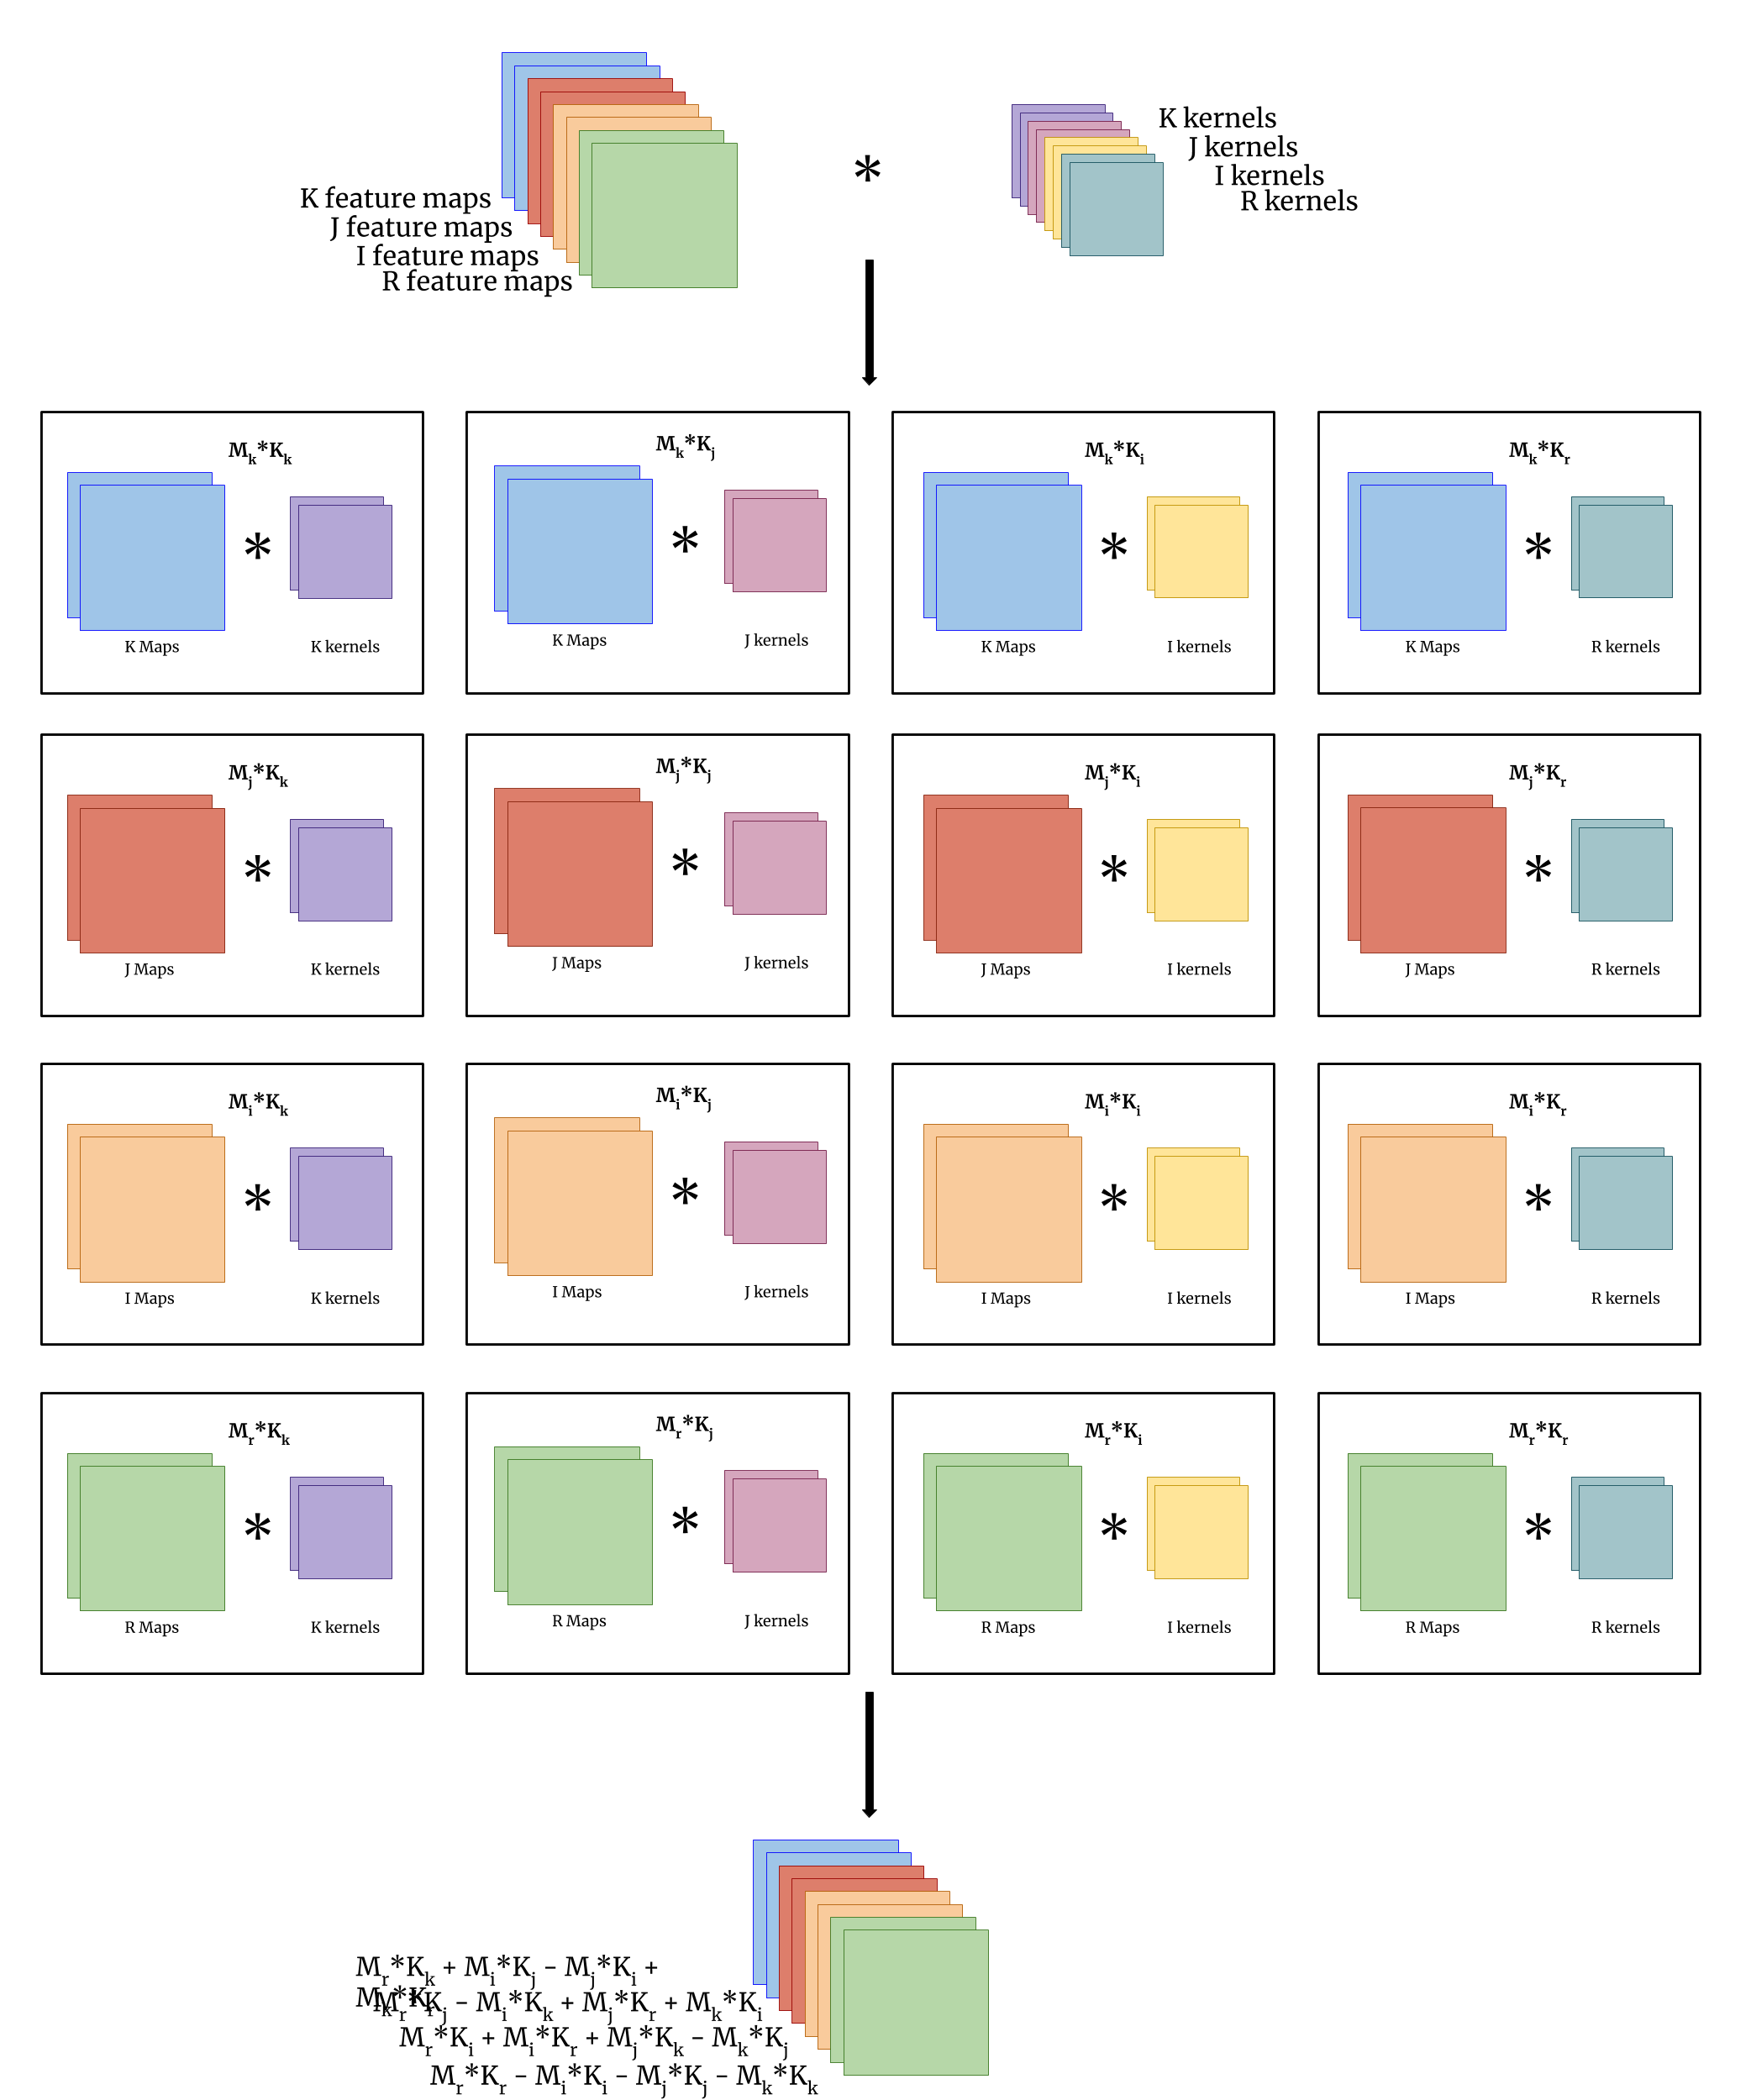
\includegraphics[width=1.0\textwidth]{figures/quatconv.png}
	\caption{An illustration of quaternion convolution.}
	\label{f:quatconv}
\end{figure*}


\subsection{Quaternion Batch-Normalization}
Batch-normalization \cite{ioffe2015batch} is used by the vast majority of all deep networks to stabilize and speed up training.
It works by keeping the activations of the network at zero mean and unit variance.
The original formulation of batch-normalization only works for real-values. 
Applying batch normalization to complex or hyper-complex numbers is more difficult, one can not simply translate and scale them such that their mean is 0 and their variance is 1.
This would not give equal variance in the multiple components of a complex or hyper-complex number.
To overcome this for complex numbers a whitening approach is used \cite{trabelsi2017deep}, which scales the data by the square root of their variances along each of the two principle components.
We use the same approach, but must whiten 4D vectors.

However, an issue arises in that there is no nice way to calculate the inverse square root of a 4~x~4 matrix.
It turns out that the square root is not necessary and we can instead use the Cholesky decomposition on our covariance matrix.
The details of why this works for whitening given in the Appendix section \ref{a:whitening}.
Now our whitening is accomplished by multiplying the \textbf{0}-centered data ($\textbf{x} - \mathbb{E}[\textbf{x}]$) by \textbf{W}:
\begin{equation}
\tilde{x} = \textbf{W}(\textbf{x} - \mathbb{E}[\textbf{x}])
\label{eq:white4d}
\end{equation}
where \textbf{W} is one of the matrices from the Cholesky decomposition of $\textbf{V}^{-1}$ where \textbf{V} is the covariance matrix given by:
\begin{align*}
\textbf{V}
=&
\begin{bmatrix}
 V_{rr} & V_{ri} & V_{rj} & V_{rk} \\
 V_{ir} & V_{ii} & V_{ij} & V_{ik} \\
 V_{jr} & V_{ji} & V_{jj} & V_{jk} \\
 V_{kr} & V_{ki} & V_{kj} & V_{kk}
\end{bmatrix} \nonumber \\
&=\left[ 
\begin{matrix*}[l]
\mbox{C}(\mathscr{R}\{\textbf{x}\}, \mathscr{R}\{\textbf{x}\}) \\
\mbox{C}(\mathscr{I}\{\textbf{x}\}, \mathscr{R}\{\textbf{x}\}) \\
\mbox{C}(\mathscr{J}\{\textbf{x}\}, \mathscr{R}\{\textbf{x}\}) \\
\mbox{C}(\mathscr{K}\{\textbf{x}\}, \mathscr{R}\{\textbf{x}\}) \\
\end{matrix*} \right. \nonumber 
\begin{matrix*}[l]
\mbox{C}(\mathscr{R}\{\textbf{x}\}, \mathscr{I}\{\textbf{x}\}) \\
\mbox{C}(\mathscr{I}\{\textbf{x}\}, \mathscr{I}\{\textbf{x}\}) \\
\mbox{C}(\mathscr{J}\{\textbf{x}\}, \mathscr{I}\{\textbf{x}\}) \\
\mbox{C}(\mathscr{K}\{\textbf{x}\}, \mathscr{I}\{\textbf{x}\}) \\
\end{matrix*} \nonumber 
\begin{matrix*}[l]
\mbox{C}(\mathscr{R}\{\textbf{x}\}, \mathscr{J}\{\textbf{x}\}) \\
\mbox{C}(\mathscr{I}\{\textbf{x}\}, \mathscr{J}\{\textbf{x}\}) \\
\mbox{C}(\mathscr{J}\{\textbf{x}\}, \mathscr{J}\{\textbf{x}\}) \\
\mbox{C}(\mathscr{K}\{\textbf{x}\}, \mathscr{J}\{\textbf{x}\}) \\
\end{matrix*} \nonumber  \left.
\begin{matrix*}[l]
\mbox{C}(\mathscr{R}\{\textbf{x}\}, \mathscr{K}\{\textbf{x}\}) \\
\mbox{C}(\mathscr{I}\{\textbf{x}\}, \mathscr{K}\{\textbf{x}\}) \\
\mbox{C}(\mathscr{J}\{\textbf{x}\}, \mathscr{K}\{\textbf{x}\}) \\
\mbox{C}(\mathscr{K}\{\textbf{x}\}, \mathscr{K}\{\textbf{x}\}) \\
\end{matrix*}  \right]
\label{eq:V4d}
\end{align*}
where C$(\cdot)$ is the covariance and $\mathscr{R}\{x\}$, $\mathscr{I}\{x\}$, $\mathscr{J}\{x\}$, and $\mathscr{K}\{x\}$ are the real, $i$, $j$, and $k$ components of $\textbf{x}$ respectively.

Real-valued batch normalization also uses two learned parameters, $\beta$ and $\gamma$. 
Our shift parameter {\boldmath$\beta$} must shift a quaternion value so it is a quaternion value itself with real, $i$, $j$, and $k$ as learnable components. 
The scaling parameter {\boldmath$\gamma$} is a symmetric matrix of size matching $\textbf{V}$ given by:
\begin{equation}
\mathbf{\gamma}
=
\left( 
\begin{array}{cccc}
V_{rr} & V_{ri} & V_{rj} & V_{rk} \\
V_{ri} & V_{ii} & V_{ij} & V_{ik} \\
V_{rj} & V_{ij} & V_{jj} & V_{jk} \\
V_{rk} & V_{ik} & V_{jk} & V_{kk}
\end{array}
\right)
\label{eq:gamma}
\end{equation}
Because of its symmetry it has only ten learnable parameters. 
The variance of the components of input $\tilde{\textbf{x}}$ are variance 1 so the diagonal of {\boldmath$\gamma$} is initialized to $1/\sqrt{16}$ in order to obtain a modulus of 1 for the variance of the normalized value. 
The off diagonal terms of {\boldmath$\gamma$} and all components of {\boldmath$\beta$} are initialized to 0.
The quaternion batch normalization is defined as:
\begin{equation}
\mbox{BN}(\tilde{\textbf{x}}) = \mathbf{\gamma}\tilde{\textbf{x}} + \mathbf{\beta}
\label{eq:qbn}
\end{equation}


\subsection{Quaternion Weight Initialization}
The proper initialization of weights is vital to convergence of deep networks. 
In this work we derive our quaternion weight initialization using the same procedure as Glorot and Bengio \cite{glorot2010understanding} and He et al. \cite{he2015delving}.

To begin we find the variance of a quaternion weight:
\begin{align}
W = &~|W|e^{(\mbox{cos}\phi_1 \textit{i} + \mbox{cos}\phi_2 \textit{j} + \mbox{cos}\phi_3 \textit{k})\theta} \nonumber \\
= &~\mathscr{R}\{W\} + \mathscr{I}\{W\} + \mathscr{J}\{W\} + \mathscr{K}\{W\}.
\label{eq:quaternion_weight}
\end{align}
where $|W|$ is the magnitude, $\theta$ and $\phi$ are angle arguments, and $\mbox{cos}^2\phi_1 + \mbox{cos}^2\phi_2 + \mbox{cos}^2\phi_3 = 1$ \cite{turner2002}.

Variance is defined as
\begin{equation}
\mbox{Var}(W) = \mathbb{E}[|W|^2] - (\mathbb{E}[W])^2,
\label{eq:variance}
\end{equation}
but since $W$ is symmetric around 0 the term $(\mathbb{E}[W])^2$ is 0. 
We do not have a way to calculate $\mbox{Var}(W) = \mathbb{E}[|W|^2]$ so we make use of the magnitude of quaternion normal values $|W|$, which follows an independent normal distribution with four degrees of freedom (DOFs).
We can then calculate the expected value of $|W|^2$ to find our variance
\begin{equation}
\mathbb{E}[|W|^2] = \int_\infty^\infty x^2 f(x) ~dx = 4\sigma^2
\label{eq:expected}
\end{equation}
where $f(x)$ is the four DOF distribution given in the Appendix.

And since $\mbox{Var}(W) = \mathbb{E}[|W|^2]$, we now have the variance of $W$ expressed in terms of a single parameter $\sigma$:
\begin{equation}
\mbox{Var}(W) = 4\sigma^2.
\label{eq:variance_sigma}
\end{equation}

To follow the Glorot and Bengio \cite{glorot2010understanding} initialization we have $\mbox{Var}(W) = 2/(n_{in}+n_{out})$, where $n_{in}$ and $n_{out}$ are the number of input and output units respectivly. 
Setting this equal to \eqref{eq:variance_sigma} and solving for $\sigma$ gives $\sigma = 1/\sqrt{2(n_{in}+n_{out})}$.
To follow He et al. \cite{he2015delving} initialization that is specialized for rectified linear units (ReLUs) \cite{nair2010rectified}, then we have $\mbox{Var}(W) = 2/n_{in}$, which again setting equal to \eqref{eq:variance_sigma} and solving for $\sigma$ gives $\sigma = 1/\sqrt{2n_{in}}$.

As shown in \eqref{eq:quaternion_weight} the weight has components $|W|$, $\theta$, and $\phi$. 
We can initialize the magnitude $|W|$ using our four DOF distribution defined with the appropriate $\sigma$ based on which initialization scheme we are following. 
The angle components are initialized using the uniform distribution between $-\pi$ and $\pi$ where we ensure the constraint on $\phi$.


\section{Experimental Results}
Our experiments covered image classification using both the CIFAR-10 and CIFAR-100 benchmarks and image segmentation using the KITTI Road Estimation benchmark.

\subsection{Classification}
We use the same architecture as the large model in \cite{trabelsi2017deep}, which is a 110 layer Residual model similar to the one in \cite{he2016deep}.
There is one difference between the real-valued network and the ones used for both the complex and hyper-complex valued networks.
Because the datasets are all real-valued the network must learn the imaginary or quaternion components.
We use the same technique as \cite{trabelsi2017deep} where there is an additional block immediately after the input which will learn the hyper-complex components
\begin{equation*}
BN \rightarrow ReLU \rightarrow Conv \rightarrow BN \rightarrow ReLU \rightarrow Conv.
\end{equation*}

Since all datasets that we work with are real-valued,
we present a way to learn their imaginary components to let the rest of the network operate in the
complex plane. 
We learn the initial imaginary component of our input by performing the operations
present within a single real-valued residual block

This means that to maintain the same approximate parameter count the number of convolution kernels for the complex network was increased.
We however did not increase the number of convolution kernels for the quaternion trials so any increase in model performance comes from the quaternion filters and at a lower hardware budget.

The architecture consists of 3 stages of repeating residual blocks where at the end of each stage the images are downsized by strided convolutions.
Each stage also doubles the previous stage's number of convolution kernels.
The last layers are a global average pooling layer followed by a single fully connected layer with a softmax function used to classify the input as either one of the 10 classes in CIFAR-10 or one of the 100 classes in CIFAR-100.

We also followed their training procedure of using the backpropagation algorithm with Stochastic Gradient Descent with Nesterov momentum \cite{nesterov1983method} set at 0.9.
The norm of the gradients are clipped to 1 and a custom learning rate scheduler is used.
The learning scheduler is the same used in \cite{trabelsi2017deep} for a direct comparison in performance.
The learning rate is initially set to 0.01 for the first 10 epochs and then set it to 0.1 from epoch 10-100 and then cut by a factor of 10 at epochs 120 and 150.
Table~\ref{t:results1} presents our results along side the real and complex valued networks.
Our quaternion model outperforms the real and complex networks on both datasets on a smaller parameter budget.

\begin{table}[h]
	\centering
		\begin{tabular}{l c c}
			\hline
			Architecture & CIFAR-10 & CIFAR-100 \\
			\hline
			\cite{he2016deep} Real & 6.37 & - \\
			\cite{trabelsi2017deep} Complex & 5.60 & 27.09 \\
			Quaternion & \textbf{5.44} & \textbf{26.01}
		\end{tabular}
	\caption{Classification error on CIFAR-10 and CIFAR-100. Note that \cite{he2016deep} is a 110 layer residual network, \cite{trabelsi2017deep} is 118 layer complex network with the same design as the prior except with additional initial layers to extract complex mappings.}
	\label{t:results1}
\end{table}

\subsection{Segmentation}
For this experiment we used the same model as the above, but cut the number of residual blocks out of the model for memory reasons given that the KITTI data is large color images.
The 110 layer model has 10, 9, and 9 residual blocks in the 3 stages talked about above, while this model has 2, 1, and 1 and does not perform any strided convolutions.
This gives a total of 38 layers.

The last layer is a $1 \times 1$ convolution with a sigmoid output so we are getting a heatmap prediction the same size as the input.
The training procedure is also as above, but the learning rate is scheduled differently.
Here we begin at 0.01 for the first 10 epochs and then set it to 0.1 from epoch 10-50 and then cut by a factor of 10 at 100 and 150.
Table~\ref{t:results2} presents our results along side the real and complex valued networks where we used Intersection over Union (IOU) for performance measure.
Quaternion outperformed the other two by a larger margin compared to the classification tasks.

\begin{table}[h]
	\centering
		\begin{tabular}{l c c}
			\hline
			Architecture & KITTI \\
			\hline
			Real & 0.747 \\
			Complex & 0.769 \\
			Quaternion & \textbf{0.827}
		\end{tabular}
	\caption{IOU on KITTI Road Estimation benchmark.}
	\label{t:results2}
\end{table}


\section{Conclusions and Proposed Research}
We have extended upon work looking into complex valued networks by exploring quaternion values.
We presented the building blocks required to build and train deep quaternion networks and used them to test residual architectures on two common image classification benchmarks.
We show that they have competitive performance by beating both the real and complex valued networks with less parameters.

Since the entirety of the work so far has been done in supervised learning, it seems prudent to explore results in unsupervised learning compared to real and complex networks.
The proposed idea is to test quaternion values in a Deep Adversarial Gaussian Mixture Autoencoder \cite{harchaoui2017deep}.
We will compare the current results of with results of both complex and quaternion networks.
Another area to explore would be in networks designed to handle 3D data given quaternions natural expressive capapilities in this area.
PointNet \cite{qi2017pointnet} and its newer variants take in a group of 3D points and use a deep network to classify the entire cloud as a class and/or classify each point in the cloud as a class.
We will compare the latest PointNet variant with complex and quaternion value models.

The majority of work was the upfront work of creating and coding the algorithms needed for deep quaternion networks.
With that done the work to explore these last two ideas only involves pulling the authors code and replacing their real layers with complex and then quaternion layers.
Including running the experiments the amount of time would be less than 6 months.